\documentclass[a4paper, twoside, 12pt]{article}
%packages
\usepackage[utf8]{inputenc}
\usepackage{graphicx}
\usepackage[]{background}
\usepackage[a4paper,top=2cm,bottom=2cm,left=2cm,right=2cm,marginparwidth=2cm]{geometry}
\usepackage[english]{babel}
\usepackage[section]{placeins}
\usepackage{enumitem}
\usepackage{float}
\usepackage[colorinlistoftodos]{todonotes}
\usepackage{multirow}
\usepackage{amsmath}
\usepackage{mathrsfs}
\usepackage{eurosym}
\usepackage{fancyhdr}
\pagestyle{fancy}
\usepackage{titlesec}
\usepackage{caption}
\usepackage{wrapfig}
\usepackage{tabularx}
\usepackage[table]{xcolor}
\usepackage{pgfplots}
\pgfplotsset{compat=1.17}
\usepackage[backend=biber, style=numeric]{biblatex}
\usepackage[colorlinks=true, linkcolor=blue, citecolor=blue]{hyperref}
\usetikzlibrary{shapes.geometric, arrows}


\linespread{1}


\renewcommand{\headrulewidth}{2pt}
\renewcommand{\sectionmark}[1]{\markboth{#1}{#1}}
\fancyhead[R]{}
\fancyhead[L]{\texttt{\leftmark}}


%\renewcommand{\familydefault}{\sfdefault}

%
\begin{document}
\begin{titlepage}

	\newcommand{\HRule}{\rule{\linewidth}{0.5mm}} % Defines a new command for the horizontal lines, change thickness here

	%----------------------------------------------------------------------------------------
	%	LOGO SECTION
	%----------------------------------------------------------------------------------------

	
\includegraphics[width=8cm]{img/logo-polytech.jpg}\\[1cm] % Include a department/university logo - this will require the graphicx package

	%----------------------------------------------------------------------------------------

	\center % Center everything on the page

	%----------------------------------------------------------------------------------------
	%	HEADING SECTIONS
	%----------------------------------------------------------------------------------------

	\textsc{\LARGE ELEC-H410}\\[1.5cm] % Name of your university/college
	\textsc{\Large Université Libre de Bruxelles}\\[0.5cm] % Major heading such as course name
	\textsc{\large École Polytechnique de Bruxelles}\\[0.5cm] % Minor heading such as course title

	%----------------------------------------------------------------------------------------
	%	TITLE SECTION
	%----------------------------------------------------------------------------------------
	\makeatletter
	\HRule \\[0.4cm]
	{ \huge \bfseries Pandemic Project}\\[0.4cm] % Title of your document
	\HRule \\[1.5cm]

	%----------------------------------------------------------------------------------------
	%	AUTHOR SECTION
	%----------------------------------------------------------------------------------------

	\begin{minipage}{0.4\textwidth}
		\begin{flushleft} \large
			\emph{Authors of Group 13:}\\ % Your name

			JANKE Nico (540076) \\ VAN Dyck Emile (540174) \\ WOJTACH Kacper (513025)
		\end{flushleft}
	\end{minipage}
	~
	\begin{minipage}{0.4\textwidth}
		\begin{flushright} \large
			\emph{Professor:} \\
			QUITIN François
		\end{flushright}
	\end{minipage}\\[2cm]
	\makeatother

	% If you don't want a supervisor, uncomment the two lines below and remove the section above
	%\Large \emph{Author:}\\
	%John \textsc{Smith}\\[3cm] % Your name

	%----------------------------------------------------------------------------------------
	%	DATE SECTION
	%----------------------------------------------------------------------------------------

	{\large \today}\\[2cm] % Date, change the \today to a set date if you want to be precise

	\backgroundsetup{scale=1,
		color=black,
		opacity=0.17,
		angle=10,
		position={12cm,-22cm},contents={%
				
\includegraphics[height=20cm,width=20cm,keepaspectratio]{img/sceauULB.jpg}}%
	}

	\vfill % Fill the rest of the page with whitespace

\end{titlepage}

\newpage
\BgThispage
\backgroundsetup{contents={}}
\tableofcontents
\newpage

\section{Introduction}
The goal of the pandemic game is to produce enough vaccines to eradicate the virus
before the population collapses. We have an interface (\texttt{pandemic.h})
to communicate with the game routine.
\begin{itemize}
	\setlength\itemsep{0em}
	\item Every 3 seconds a vaccine clue is dropped.
	\item Every 5 seconds, the percentage of healthy people in the population is updated.
	\item On random occasions, an individual gets contaminated, and we need to quarantine the population in less than 10 milliseconds.
\end{itemize}
To manage these events and win the game, we created one task for each with different
priorities. We also have a task dedicated to printing the state of the game on a LCD screen.

\section{Tasks and Synchronization}
\subsection{Quarantine}
This task has the highest priority of all our tasks. All it does is wait for the
\texttt{QuarantineStart} binary semaphore to be available. This is triggered by contamination.
When the semaphore is available, the task starts the quarantine. This is done on time because
of the priority of the task.

\subsection{Vaccine}
The \texttt{vaccineProductionTask} has the third highest priority. It waits for a clue to be
released and the \texttt{lab} semaphore to be freed to start producing a vaccine.
That way we start producing as soon as we get a clue. This is needed because we have 3 seconds to produce a vaccine after release. If we need to wait on the lab for more than 475ms we decide to not start the vaccine production because we will not have the time to do it.\\
When the vaccine is produced, we ship it immediately. Once this is done, we give the \texttt{lcd}
and \texttt{lab} semaphores. The first one is to notify the LCD task that the game state has changed,
and the second one is to notify the Medicine task that it can produce or ship a medicine.

\subsection{Medicine}
In order to alternate between producing and shipping the medicine, the \texttt{medicineProductionTask} contains two consecutive sections, each beginning by waiting for the \texttt{lab} semaphore and ending by releasing it. The first one handles production, and the second one handles shipping. Since it has a lower priority, it will only run if \texttt{vaccineProductionTask} is waiting for the \texttt{vaccineStart} semaphore.
This will be more visible in the logic analyzer traces.


\subsection{LCD}
The last task has the second highest priority. This is needed because if it is not the case the LCD will never update. It is notified by the vaccine and medicine tasks when the game state has changed. It will print the state of the game as specified in the
specification.



\section{Logic Analyzer Traces}

\subsection{Startup and Periodic Execution}
Fig.\ref{fig:start_and_periodic} shows the early behavior of the FreeRTOS-based pandemic simulation. The six digital signals (D0–D5) represent GPIO pins toggled by specific tasks:


\begin{itemize}
	\setlength\itemsep{0em}
	\item D0: \texttt{releaseContamination} + \texttt{quarantineTask}
	\item D1: \texttt{medicineProductionTask} : Production segment
	\item D2: \texttt{medicineProductionTask} : Shipping segment
	\item D3: \texttt{vaccineProductionTask}
	\item D4: \texttt{lcdTask}
	\item D5: \texttt{releaseClue}
\end{itemize}


\begin{figure}[ht!]
	\centering
	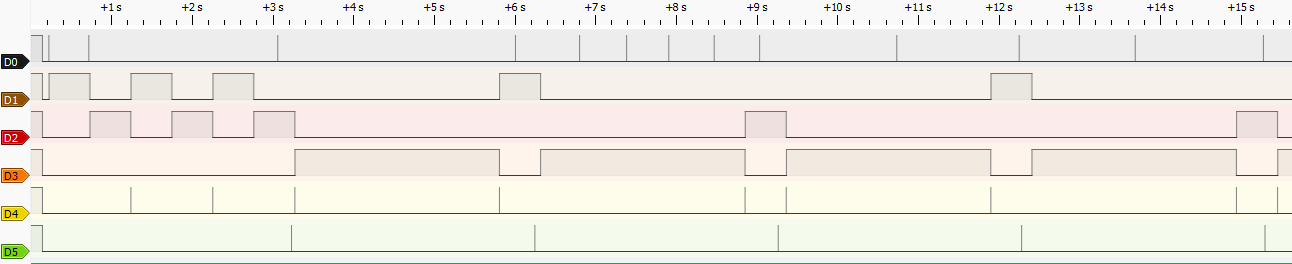
\includegraphics[width=1.05\linewidth]{../run_pulseview/start_and_periodic_part2.png}
	\caption{Early Behavior of the simulation}
	\label{fig:start_and_periodic}
\end{figure}

\subsubsection{Startup Phase}
At the beginning of the trace, all signals are low. This shows that the system starts in a clean and reset state.\\
Immediately after startup:
\begin{itemize}
	\setlength\itemsep{0em}
	\item D1 (Medicine Production) goes high, indicating that the medicine production task runs first
	      \begin{itemize}
		      \setlength\itemsep{0em}
		      \item This matches the behavior in the code: \texttt{medicineProductionTask()} runs in a loop and starts as soon as it can get the lab mutex.
	      \end{itemize}
	\item Then D2 (Medicine Shipment) is activated, showing that the medicine is shipped.
	\item D4 (LCD Update) follows, confirming that the LCD is refreshed right after the medicine shipment — triggered by xSemaphoreGive(lcd) in the medicine task.

\end{itemize}
.
There is no sign of D5 (Clue Release) or D3 (Vaccine Production) at the beginning, meaning the game task hasn't triggered a clue yet.

\subsubsection{Periodic Execution}
Later in the trace, a regular pattern begins:
\begin{itemize}
	\setlength\itemsep{0em}
	\item D5 – Clue Release: The game task releases a clue using \texttt{releaseClue()}.
	\item D3 – Vaccine Production: The vaccine task picks up the clue, produces a vaccine, and gives the LCD semaphore.
	\item D4 – LCD Update: The display is updated with the new vaccine, medicine, population counters.
	\item D1/D2 – Medicine Production/Shipment: If allowed, the medicine is produced again/After production, the medicine is shipped.
	\item D4 – LCD Update: Again, the LCD is refreshed.
\end{itemize}

\subsubsection{Aperiodic Contamination Events}
Around t = 0.7s, D0 goes high: a contamination is released and the quarantine task is executed.
\begin{itemize}
	\setlength\itemsep{0em}
	\item This does not follow a fixed interval, confirming that contamination is aperiodic, as controlled by game logic in the gameTask.
\end{itemize}


This full loop repeats roughly every 3 seconds, showing synchronized task execution using FreeRTOS semaphores and mutexes.

\subsection{Timing Drift Due to Contaminations and Mutex Timeout Limit}

\begin{figure}[ht!]
	\centering
	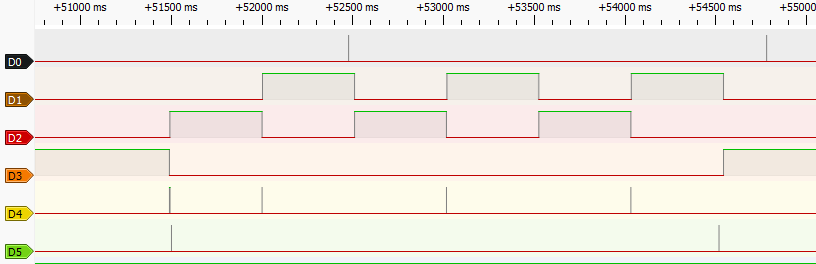
\includegraphics[width=1\linewidth]{../run_pulseview/delayed2.png}
	\caption{Reset of the "periodicity" during the simulation}
	\label{fig:delayed}
\end{figure}

In the observed trace (Fig.\ref{fig:start_and_periodic}), the system initially maintains a regular cycle of medicine production (D1), shipment (D2), clue release (D5), and vaccine production (D3). However, this periodicity is disrupted over time due to delays caused by the aperiodic contamination events (D0), the lcd task (D4) and the OS itself.\\
Each contamination triggers the quarantine task, which preempts other tasks due to its high priority. This causes delays in the execution of lower priority tasks, such as medicine production (D1), shipment (D2), vaccine production (D3), and LCD updates (D4). As this delay accumulates, the system eventually reaches a point where the clue is released more than 475 ms before the end of an ongoing shipment or medicine production.

Since \texttt{vaccineProductionTask()} waits for access to lab mutex (shared with the production and shipment of medications), it may miss its 475-ms time-out window. When this happens (see Fig.\ref{fig:greater_than_475ms}), the vaccine task cannot start immediately after the clue release, breaking the original rhythm.\\
This resets the alignment between the drop of the clue and the start of the vaccine production. After that, the drift builds up again and causes another shift.
This phenomenon is visible in the trace in Fig.\ref{fig:delayed}:
\begin{itemize}
	\setlength\itemsep{0em}
	\item In earlier cycles, the delay between D5 (clue) and D1 or D2 is lower than 475 ms (see Fig.\ref{fig:lower_than_475ms}), so a vaccineProduction will follow.
	      \begin{figure}[ht!]
		      \centering
		      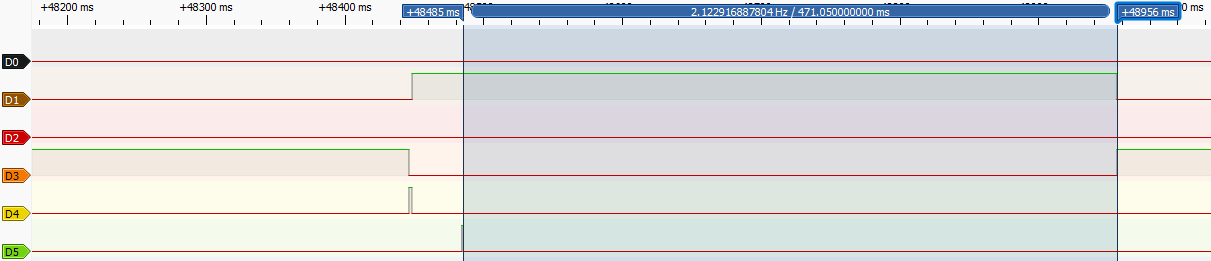
\includegraphics[width=1.05\linewidth]{../run_pulseview/lower_than_475_ms.png}
		      \caption{Time between the release of the clue and the end of the medicine production/shipment is lower than 475ms.}
		      \label{fig:lower_than_475ms}
	      \end{figure}

	\item At a critical point, this delay becomes greater than 475 ms(Fig.\ref{fig:greater_than_475ms}), causing the vaccine task to miss the mutex and restart the timing cycle.(Fig.\ref{fig:delayed})

	      \begin{figure}[ht!]
		      \centering
		      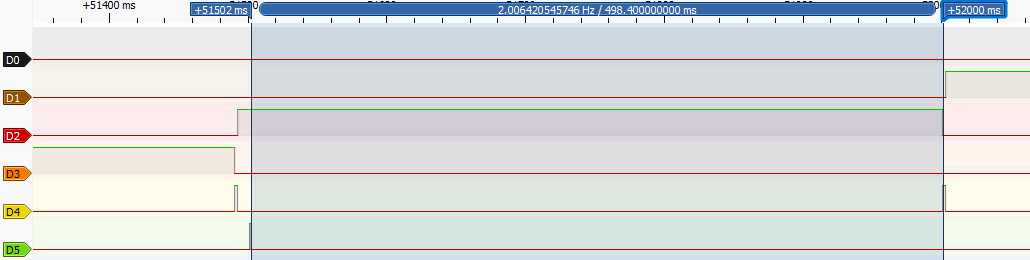
\includegraphics[width=1.05\linewidth]{../run_pulseview/greater_than_475_ms.png}
		      \caption{An instance in which the duration between clue release and shipment completion exceeds 475 ms. Therefore, the vaccineProduction related to this clue is skipped.}
		      \label{fig:greater_than_475ms}
	      \end{figure}
\end{itemize}


\newpage
\section{Conclusion}

At the end of the simulation after around 111 seconds, the system displays (Fig.\ref{fig:end_results}) a win and the three game variables.\\
These results confirm that our use of FreeRTOS tasks, priorities, and synchronization mechanisms allowed us to respond efficiently to both periodic and aperiodic events throughout the simulation.\\
The code can be found in our Github repo: \url{https://github.com/kw0jtach/RTOS_Pandemic_Project}



\begin{figure}[ht!]
	\centering
	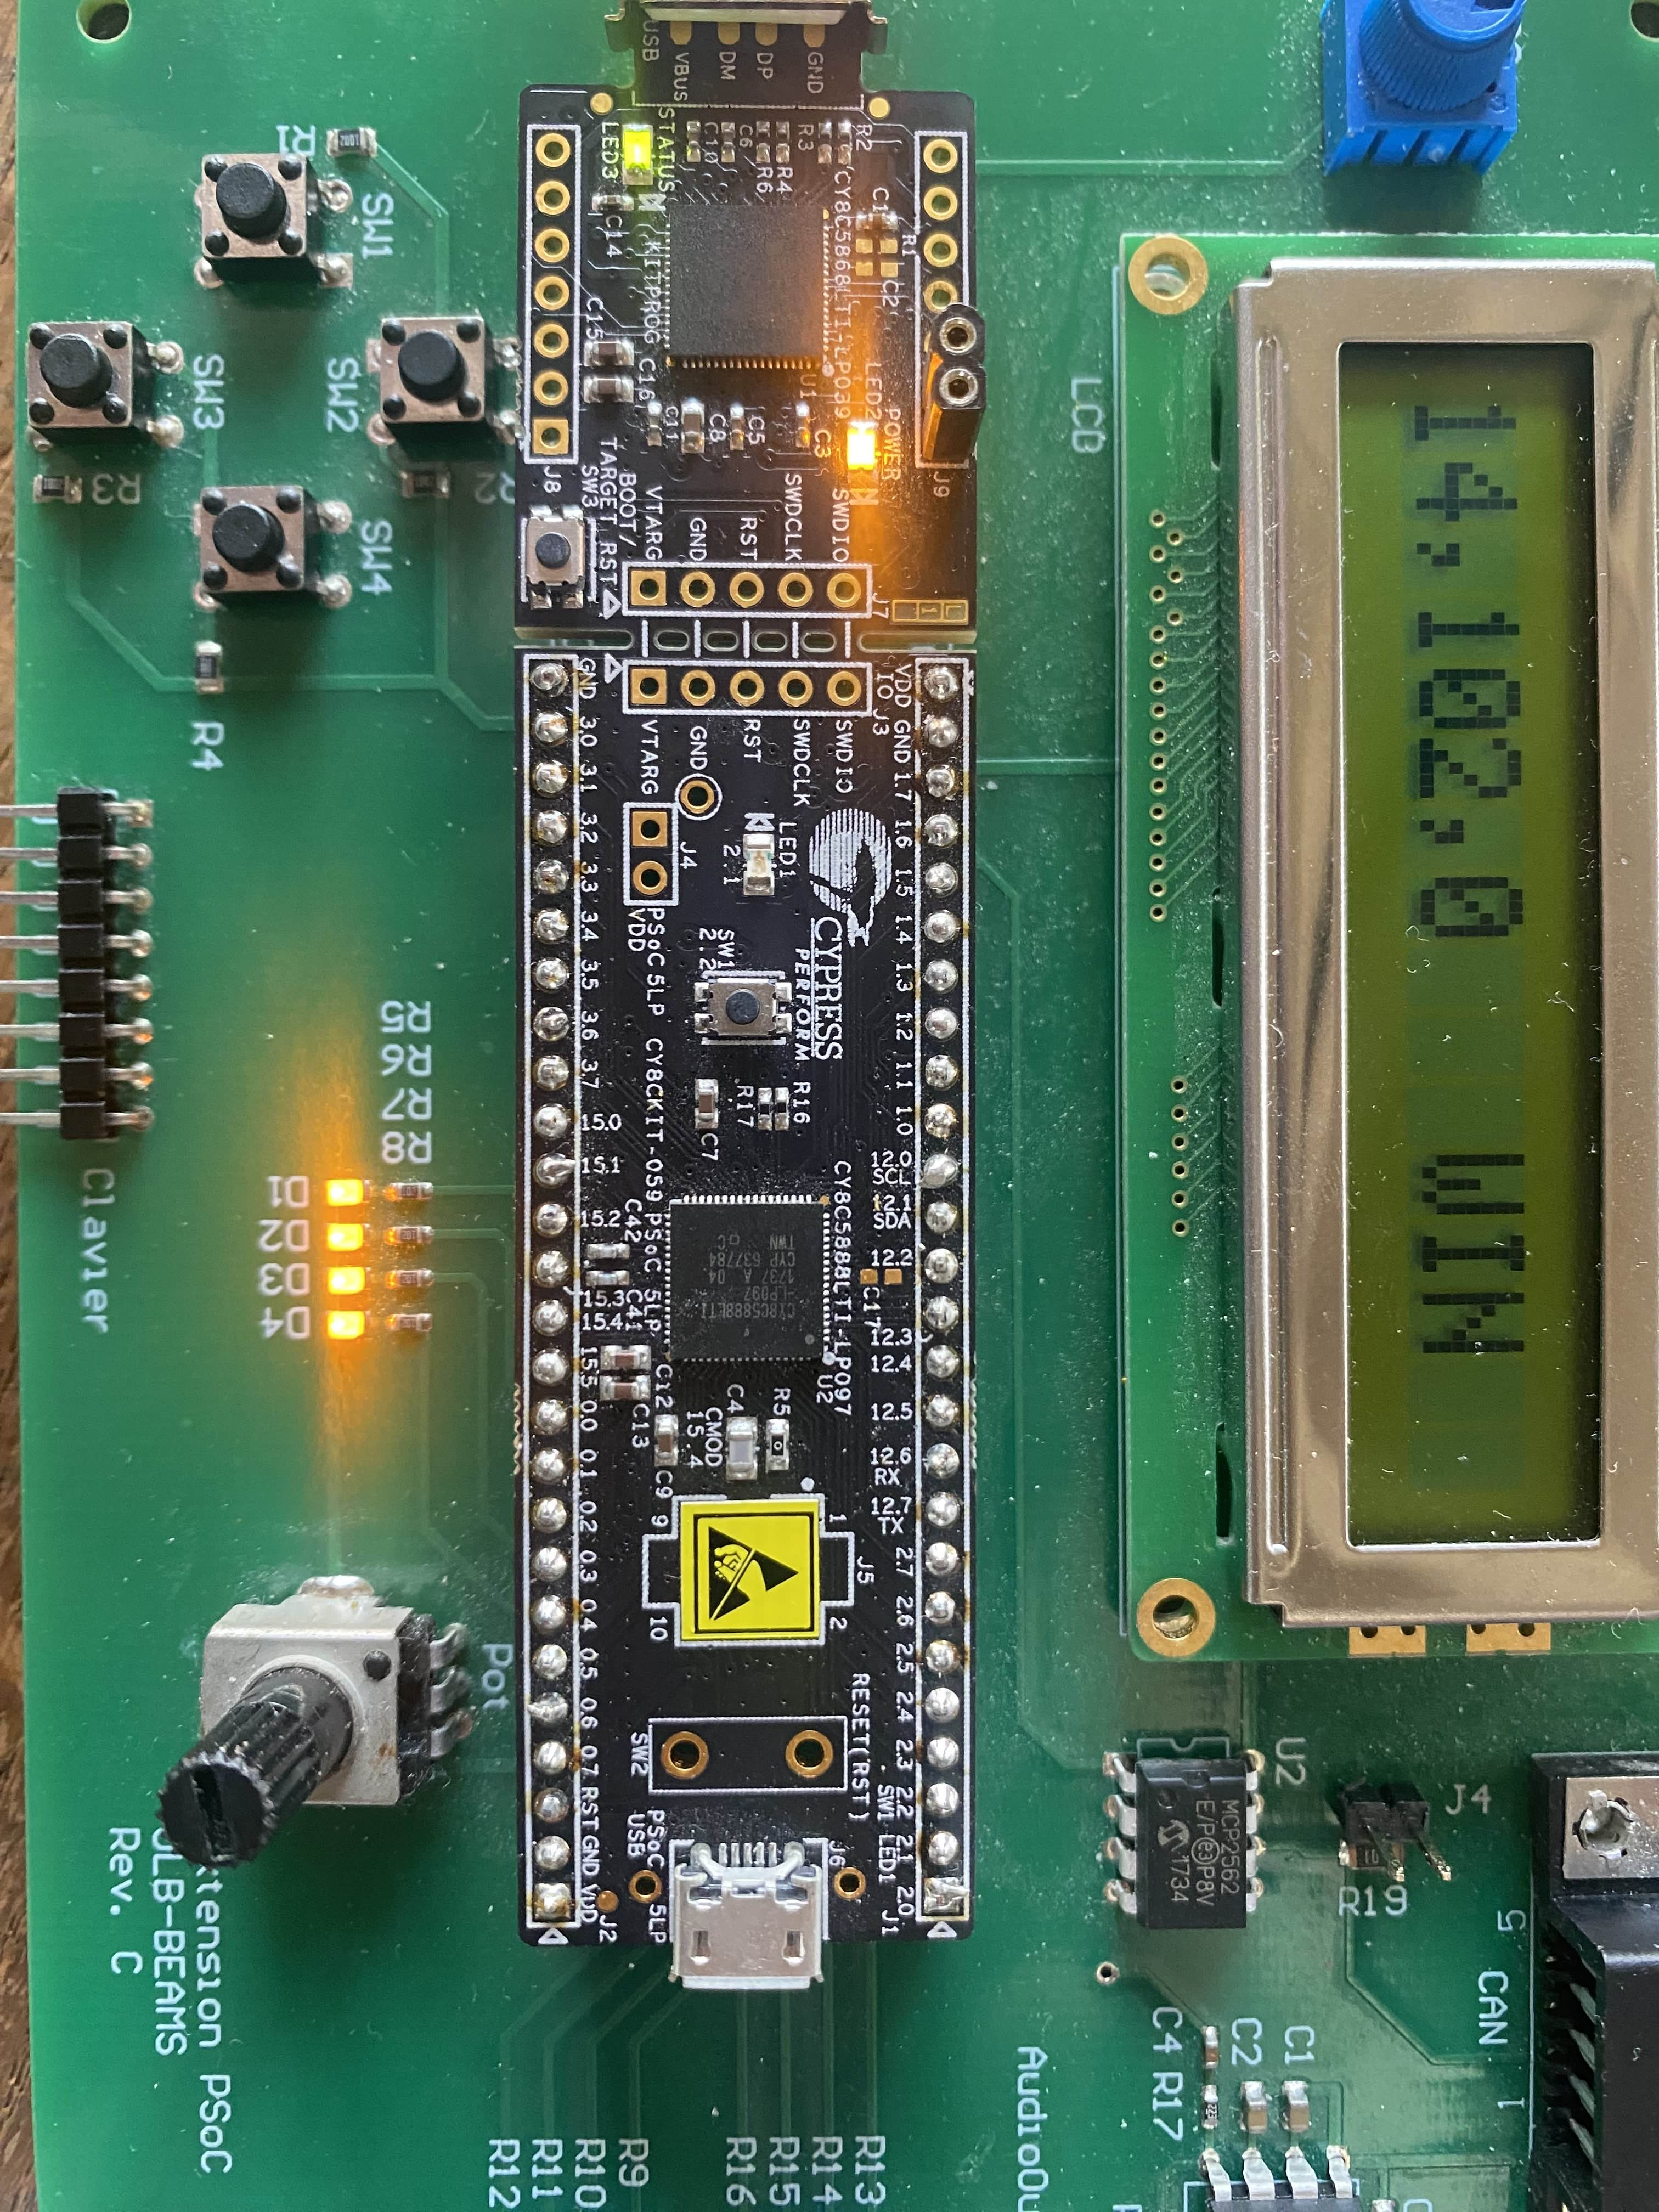
\includegraphics[width=0.5\linewidth, angle=90]{img/end_results.jpg}
	\caption{End Results}
	\label{fig:end_results}
\end{figure}

\nocite{*}
\end{document}
